\documentclass[10pt,a4paper]{book}
\usepackage[utf8]{inputenc}
\usepackage[italian]{babel}
\usepackage{amsmath}
\usepackage{amsfonts}
\usepackage{amssymb}
\usepackage{graphicx}
\usepackage{listings}
\usepackage[left=2cm,right=2cm,top=2cm,bottom=2cm]{geometry}
\author{HangaBot}
\title{Tecnologie, Disegno e Progettazione}
\begin{document}
\maketitle
\tableofcontents

\chapter{Componenti passivi}
\section{Induttori}
\section{Induttori accoppiati}
\section{Condensatori}


\chapter{Risonatori}
\section{Introduzione}
I risonatori sono dispositivi che sono accordati ad una sola frequenza o ad un numero discreto di frequenze dette frequenze di risonanza. I risonatori si possono considerare come dei filtri a banda strettissima accordati ad un numero discreto di frequenze.
Esistono risonatori a singola porta in cui la funzione di trasferimento è il parametro $S11$ e risonatori a doppia porta in cui la funzione di trasferimento è $S21$
\section{Risonatori RLC}
I risonatori RLC sono realizzati con condensatori e induttori. Questi risonatori tipicamente si usano fino alle decine di MHz. Esistono due topologie: \emph{serie} e \emph{parallelo}
\subsection{Risonatori RLC parallelo}
Nei risonatori RLC in configurazione parallelo l 'induttanza e la capacità sono collegate in parallelo.
La frequenza di risonanza è pari a
\begin{equation}
\omega_0 = \frac{1}{L C}
\end{equation}
mentre il fattore di qualità 
\begin{equation}
Q = \omega_0 R C
\end{equation}
per cui fissata la frequenza di risonanza, il fattore di qualità aumenta all' aumentare della capacità. Naturalmente l'induttanza diminuisce di conseguenza.
La banda del risonatore a metà potenza è
\begin{equation}
BW  = \frac{1}{Q}
\end{equation}
In questa topologia per ottenere dei valori di Q elevato è necessario avere dei condesatori di capacità elevata e induttanza molto piccole. Per valori di frequenza dell' ordine dei megaHerz le induttanza risultano essere troppo piccole da essere realizzate in modo controllato. 
\subsection{Risonatori RLC serie}
Nei risonatori RLC in configurazione parallelo l 'induttanza e la capacità sono collegate in parallelo.
La frequenza di risonanza è pari a
\begin{equation}
\omega_0 = \frac{1}{L C}
\end{equation}
mentre il fattore di qualità 
\begin{equation}
Q = \frac{\omega_0 L}{R}
\end{equation}
per cui fissata la frequenza di risonanza, il fattore di qualità aumenta all' aumentare della induttanza. Naturalmente la capacita  diminuisce di conseguenza.
La banda del risonatore a metà potenza è
\begin{equation}
BW  = \frac{1}{Q}
\end{equation}

\section{Risonatori con induttori accoppiati}
\section{Risonatori con linee di trasmissione}


\chapter{Analisi Spettrale di un Segnale  Campionato}
\section{Introduzione}
Supponiamo di avere un segnale $x(t)$  campionato con frequenza di campionamento $T_c$. Il numero di campioni prelevati è pari a $N$. Assumiamo, inoltre, che il segnale $x(t)$ rappresenti una tensione elettrica prelevata ai capi di una impedenza a $Z_0 = 50\Omega$ cosi da poter definire delle grandezze dimensionali. Assumiamo il segnale $x(t)$ a banda stretta e che non sia presente aliasing dello spettro.
\section{Definizioni}
Essendo il segnale campionato sono disponibili solo i campioni. La prima operazione che occorre fare è quella di ricostruire nel modo migliore possibile il segnale originario. 
Per far ciò si può utilizzare un filtro formatore di impulso che per ogni campione associa un impulso. 
Il segnale $x(t)$ può essere pertanto scritto nel seguente modo
\begin{equation}
x(t) = \sum_{n = -\infty}^{+\infty} x_n p(t-n t_c)
\end{equation}
Naturalmente $p(0) = 1$ mentre $p(n T_c) = 0 \,\forall n \neq 0$.
La trasformata di Fourier di questo segnale si scrive come 
\begin{equation}
X(f) = \int_{-\infty}^{+\infty} x(t) \exp(-j 2 \pi f t) dt
\end{equation}
Nel caso reale il numero di campioni prelevati è finito 
\begin{equation}
x_c(t) = \sum_{n = 0}^{N} x_n p(t-n t_c)
\end{equation}
In questi campioni può essere presente una periodicità e quindi un certo numero di periodi. Naturalmente quello che ci interessa è stimare lo spettro $X(f)$ a partire dalla versione limitata del segnale $x_c$. Quindi si vogliono evidenziare delle periodicità. Oppure per segnali impulsivi si vuole analizzare lo spettro come se non ci fossero altri impulsi.
Calcoliamo lo spettro del segnale $x_c(t)$ si ottiene 
\begin{equation}
X_c(t) = \int_{-\infty}^{+\infty} \left(\sum_{n = 0}^{N} x_n p(t-n t_c)\right) \exp(-j 2 \pi f t) dt
\end{equation}
portando fuori la sommatoria 
\begin{equation}
X_c(t) = \sum_{n = 0}^{N} x_n \int_{-\infty}^{+\infty} p(t-n t_c) \exp(-j 2 \pi f t) dt
\end{equation}
sfruttando la traslazione della trasformata di Fourier sia ottiene 
\begin{equation}
X_c(f) = \sum_{n = 0}^{N} x_n \exp(-j 2 \pi f n t_c)\int_{-\infty}^{+\infty} p(t) \exp(-j 2 \pi f t) dt
\end{equation}
Indicando con $P(f)$ la trasformata dell'impulso formatore si ottiene
\begin{equation}
X_c(f) = P(f)\sum_{n = 0}^{N} x_n \exp(-j 2 \pi f n t_c)
\end{equation}
ora supponiamo di volere calcolare  lo spettro in un numero discreto di frequenze cosi per utilizzare una FFT. Vista la definizione della FFT conviene scegliere

\begin{equation}
f_k = \frac{k}{N t_c} + \frac{b}{t_c}
\end{equation}

dove $b$ è un intero, e tenendo conto della periodicitò dell' esponenziale si ottiene 

\begin{equation}
X_c(f_k) = P(f_k)\sum_{n = 0}^{N} x_n \exp \left(-j 2 \pi  \frac{k}{N} n \right)
\end{equation}

Naturalmente la scelta di utilizzare quelle frequenze non è vincolante sulla risoluzione in frequenza perchè si possono sempre inserire dei campioni nulli nella sequenza ed aumentare la risoluzione.

Notiamo che il segnale $x_c(f) = x(t) rect(\frac{t - N/2 t_c}{N t_c})$ per cui lo spettro 
\begin{equation}
X_c(f) = N t_c sinc\left(f N t_c\right) \exp \left(-j 2 \pi f N/2 t_c\right ) * X(f)
\end{equation}
Quindi lo spettro del segnale troncato risulta filtrato da un filtro con risposta impulsiva pari ad una funzione sinc con una risoluzione in frequenza pari ad $1/ N t_c$. Per eliminare l' effetto della convoluzione occorre dividere per $N Tc$

\section{Calcolo densità spettrale di potenza}
Lo densità spettrale di potenza si definisce a partire dalla  autocorrelazione. Nel seguito terremo conto che il segnale è visto all'interno di una finestra di periodo $T = N T_c$ per cui l'autocorrelazione media è definita
\begin{equation}
R_x(\tau) = E \left [ \frac{1}{ T} \int_{0}^T x(t)x(t-\tau) dt \right ] 
\end{equation}
Infatti la potenza media del segnale è data da 
\begin{equation}
P_{x} = E\left[ \frac{1}{ T} \int_{0}^T {\left|x(t)\right|}^2 dt \right ]=R_{x}(0)
\end{equation}
Si definisce densità spettrale di potenza la trasformata di Fourier della funzione di autocorrelazione
\begin{equation}
S_{x}(f) = \int_{-\infty}^{\infty}R_{x}(\tau) \mathtt{e}^ {-j 2 \pi f \tau} d\tau
\end{equation}
Il motivo di questa definizione si basa sul teorema di Parseval infatti si ha che 
\begin{equation}
P_{x} = R_{x}(0) = \int_{-\infty}^\infty S_{x}(f) df
\end{equation}
La densità spettrale può essere espressa mediante lo spettro del segnale misurato si può scrivere che nel caso del segnale troncato che 

\begin{equation}
R_c(\tau) = \int_{-\infty}^{\infty}  x_c(t)x_c(t- \tau) dt
\end{equation}

si noti che 
\begin{equation}
\int_{-\infty}^{\infty} R_T(\tau) \exp(-j 2 \pi f \tau) d\tau = {\|X_c(f)\|}^2
\end{equation}

dividendo per $T$ ed effettuando la media statistica
\begin{equation}
\int_{-\infty}^{\infty} E\left[ \frac{1}{T} R_T(\tau)\right ] \exp(-j 2 \pi f \tau) d\tau = \frac{1}{T} E \left[ {\|X_c(f)\|}^2 \right]
\end{equation}

calcoliamo separatamente 
\begin{equation}
E\left[ \frac{1}{T} R_T(\tau)\right ] = \int_{-\infty}^{\infty} w_T(t) w_T(t- \tau) E \left[  	x(t)x(t - \tau)\right] = R_x(\tau) \Lambda_{T}(\tau)
\end{equation}
dove $\Lambda_{T} (\tau)$ è l' impulso triangolare che vale 1 in zero e decade a zero per $|t| <T	$
Nell'ultimo passaggio si è assunto che il il segnale misurato fosse ergodico.  
Effettuando la trasformata si ottiene che
\begin{equation}
S_x(f)*F[\Lambda_{T} (\tau)] =  \frac{1}{T} E\left[ {\|X_c(f)\|}^2\right ]
\end{equation}
ovvero 
\begin{equation}
S_x(f)* \mathrm{sinc}^2\left(f T\right) =  \frac{1}{T^2} E\left[ {\|X_c(f)\|}^2\right ]
\end{equation}
quindi effettuando la media statistica su un numero elevato di misure finestrate si ottiene la densità spettrale di potenza filtrata con un filtro a forma di sinc quadra.


\chapter{Antenne}
\section{Simulazione di antenne 4NEC2}
In 4NEC2 le antenne e le strutture sono sempre modellizzate con attraverso wire conduttori. Ogni wire è identificato da un unico tag. Durante la simulazione i wire vengono ulteriormente suddivisi dal software stesso. Quando si costruisce un modello la dimensione tipica dovrebbe essere di circa $\lambda/20$. Si possono usare segmenti di dimensione diversa per aumentare la velocità di simulazione. Occorre comunque mettere segmenti di dimensione inferiore nelle aree critiche. Per una corretta simulazione la lunghezza del segmento dovrebbe essere almeno quattro volte il diametro del conduttore.
\section{Modellizzazione di strutture solide}
In generare dei gap tra i wire inferiori a $\lambda/10$ tendono a comportarsi come un solido.
\section{Sorgenti}
In nec sono disponibili delle sorgenti di tensione ideali. I generatori di tensione si posizione al centro  dei segmenti. I generatori di tensione sono assunti infinitesimamente piccoli e non introducono gap nella geometria.
\section{Struttura del programma 4NEC2}
4NEC2 usa delle "cards" per la descrizione della simulazione. Le "cards" devono essere introdotte in un certo ordine come mostrato nella figura

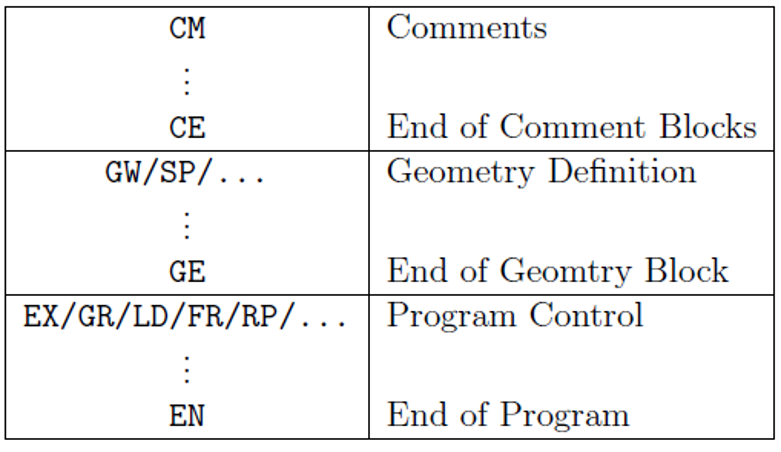
\includegraphics[scale=0.5]{img/Antenne/4NEC2_Card_Structure.png} 

\section{Esempi}
\subsection{Dipolo a $Lambda/2$ in banda X}
\lstinputlisting{labs/Antenne/4nec2/dipole.nec}

\subsection{Square loop antenna for 1 GHz}
\lstinputlisting{labs/Antenne/4nec2/square_loop.nec}

\section{Loop antenna}
\section{Introduzione}
Le antenne a loop consistono in avvolgimenti di varia forma alimentati in un punto detto gap.  In base alla loro dimensione rispetto alla lunghezza d'onda si differenziano i due tipologie

\begin{itemize}
\item Small loop - piccole rispetto alla lunghezza d'onda di funzionamento
\item Fullwave  - di dimensioni paragonabili alla lunghezza d'onda di funzionamento
\end{itemize}

Le antenne full wave ha il massimo di radiazione nella direzione ortogonale al piano dei conduttori. Le antenne small loop hanno il massimo di radiazione nel piano dei conduttori.

Sono tipicamente antenne a banda stretta con una banda tipicamente inferiore al dipolo a $\lambda/2$

\section{Loop Antenne FullWave}
Esistono diverse forme di antenna come mostrate in figura. Tipicamente La lunghezza dell'avvolgimento è pari alla lunghezza d'onda alla frequenza di funzionamento.
\begin{center}
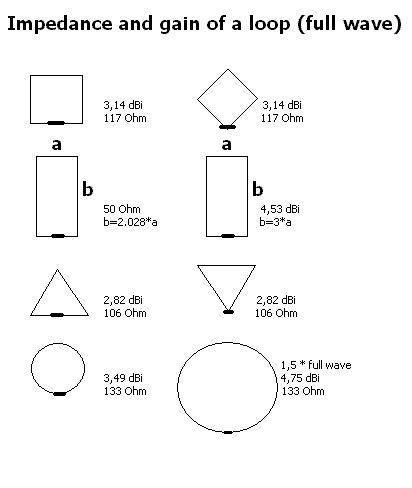
\includegraphics[scale=1]{img/Antenne/Loop_and_quad.png} 
\end{center}

\subsection{Esempio: antenna rettangolare con impedenza a 50 Ohm per la banda di 1 GHz}
La lunghezza d'onda è pari a $\lambda = 0.29979246 m$. Risolvendo il sistema
\begin{eqnarray}
2 b + 2 a = \lambda \\
b = 2.028 a
\end{eqnarray}

si ottiene 
\begin{eqnarray}
a= 0.0495 \\
b= 0.1003
\end{eqnarray}

Il codice 4NEC2 per simulare l'antenna è 
\lstinputlisting{labs/Antenne/4nec2/rectangular_loop.nec}

dalla simulazione si trova che l'antenna risulta 
\begin{center}
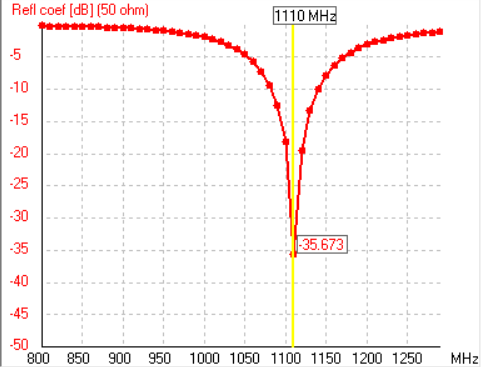
\includegraphics[scale=1]{img/Antenne/rectangular_loop_return_loss.png} 
\end{center}

Si nota che per accordare l'antenna ad 1GHz è stato previsto un fattore di scala $c$ che la rende leggermente più lunga


\chapter{Gestione di Progetto}
\section{Gestione dei Requisiti}
I requisiti di progetto sono una descrizione che mostra gli elementi e le funzioni necessarie ad un progetto. I requisiti si possono considerare come il punto di partenza di un processo di sviluppo. Quando i requisiti si modificano dopo un processo di sviluppo allora si parla di ingegneria inversa.
I requisiti si possono classificare nelle seguenti categorie
\begin{itemize}
\item Requisiti di Progetto: specificano le opzioni per un progetto
\item Requisiti di Implementazione: Specificano le tecnologie da utilizzare
\item Requisiti di Interfaccia: Specificano il modo con cui il sistema comunica con l'esterno
\item Requisiti di Forma: Specificano la forma, il peso, le dimensioni ecc
\item Requisiti di Realizzazione: Specificano i costi di realizzazione
\end{itemize}

\subsection{Analisi dei requisiti e matrice dei requisiti}
L'analisi dei requisiti  consiste nel generare un insieme di procedure di verifica automatiche o manuali che permettono di verificare se un determinato requisito è soddisfatto o meno. 

\subsection{matrice di Tracciabilità}
La matrice di tracciabilità permette di conoscere se un determinata procedura di test valuta un determinato requisito e se eseguendo la procedura si soddisfa il requisito. Naturalmente una procedura di test può andare a valutare differenti requisiti.

\section{mailbox di progetto}
La mailbox di progetto costituisce una cronologia di tutte le informazioni che vengono scambiate verso il cliente finale del progetto. Ciascun elemento nella mailBox deve generare uno o piu task che vengono messi nella task Box

\subsection{task box}
Contiene la lista dei task


\end{document}